% ============================================================================
% EVALUASI TENGAH SEMESTER — PEMROGRAMAN KONTROLLER
% BAGIAN B: STUDI LITERATUR & SIMULASI METODE BARU
% ============================================================================
\documentclass[12pt,a4paper]{article}

% ── Packages ─────────────────────────────────────────────────────────────────
\usepackage[utf8]{inputenc}
\usepackage[T1]{fontenc}
\usepackage[indonesian]{babel}
\usepackage{geometry}
\geometry{margin=2.5cm}
\setlength{\headheight}{14.5pt}
\addtolength{\topmargin}{-2.5pt}
\usepackage{graphicx}
\usepackage{longtable}
\usepackage{booktabs}
\usepackage{array}
\usepackage{hyperref}
\usepackage{enumitem}
\usepackage{amsmath}
\usepackage{tikz}
\usetikzlibrary{shapes.geometric, arrows.meta, positioning, fit, calc}
\usepackage{listings}
\usepackage{xcolor}
\usepackage{float}
\usepackage{caption}
\usepackage{subcaption}
\usepackage{fancyhdr}

% ── Listing Style untuk Rust ─────────────────────────────────────────────────
\definecolor{rustbg}{RGB}{40,40,40}
\definecolor{rustfg}{RGB}{220,220,200}
\definecolor{rustkw}{RGB}{249,174,88}
\definecolor{rustcm}{RGB}{106,153,85}
\definecolor{ruststr}{RGB}{206,145,120}
\lstdefinelanguage{Rust}{
  keywords={fn, let, mut, if, else, loop, struct, static, const, use, pub, mod, impl, return, true, false, unsafe, extern, crate, self, super, as, break, continue, for, in, match, ref, type, where, while, async, await, move},
  morecomment=[l]{//},
  morecomment=[s]{/*}{*/},
  morestring=[b]",
  sensitive=true,
}
\lstset{
  language=Rust,
  basicstyle=\ttfamily\footnotesize\color{rustfg},
  backgroundcolor=\color{rustbg},
  keywordstyle=\color{rustkw}\bfseries,
  commentstyle=\color{rustcm}\itshape,
  stringstyle=\color{ruststr},
  numbers=left,
  numberstyle=\tiny\color{gray},
  frame=single,
  rulecolor=\color{gray},
  breaklines=true,
  tabsize=4,
  showstringspaces=false,
}

% ── Header/Footer ───────────────────────────────────────────────────────────
\pagestyle{fancy}
\fancyhf{}
\rhead{ETS Pemrograman Kontroller 2025/2026}
\lhead{Bagian B: Studi Literatur \& Simulasi}
\cfoot{\thepage}

% ── Hyperlink Style ──────────────────────────────────────────────────────────
\hypersetup{
  colorlinks=true,
  linkcolor=blue!70!black,
  citecolor=blue!70!black,
  urlcolor=blue!60!black,
}

% ═══════════════════════════════════════════════════════════════════════════════
\begin{document}

% ── Halaman Sampul ───────────────────────────────────────────────────────────
\begin{titlepage}
\centering
\vspace*{2cm}
{\LARGE\bfseries EVALUASI TENGAH SEMESTER\\[0.3cm]}
{\Large MATA KULIAH PEMROGRAMAN KONTROLLER\\[0.5cm]}
{\large BAGIAN B: STUDI LITERATUR \& SIMULASI METODE BARU\\[1.5cm]}
\rule{\linewidth}{0.5pt}\\[0.5cm]
{\huge\bfseries Safe-Concurrency for\\Multi-Sensor Fusion in\\Industrial Safety-Critical Systems\\[0.5cm]}
\rule{\linewidth}{0.5pt}\\[1.5cm]
{\large Disusun oleh:\\[0.5cm]}
{\Large Abdurrauf Almutawakkil\\NRP:  2042241115\\[0.3cm]}
{\large Kelas: 4C\\[0,5cm]}
{\large Dosen Pengampu:\\[0.3cm]}
{\large Ahmad Radhy, S.Si., M.Si.\\[1.5cm]}
Program Studi Rekayasa Teknologi Instrumentasi\\
Semester Genap 2025/2026\\[2cm]
3 Mei 2026
\end{titlepage}

\tableofcontents
\newpage

% ═══════════════════════════════════════════════════════════════════════════════
\section{Studi Literatur}
% ═══════════════════════════════════════════════════════════════════════════════

% sections/tabel_jurnal.tex — Tabel Ringkasan 25 Jurnal Acuan
\begin{small}
\newcolumntype{C}[1]{>{\centering\arraybackslash}m{#1}}
\begin{longtable}{|c|C{3.2cm}|C{2cm}|C{2.5cm}|C{2.5cm}|C{2.8cm}|}
\hline
\textbf{No} & \textbf{Judul Artikel} & \textbf{Penulis (Tahun)} & \textbf{Metode} & \textbf{Hasil Utama} & \textbf{Future Work} \\
\hline
\endfirsthead
\hline
\textbf{No} & \textbf{Judul Artikel} & \textbf{Penulis (Tahun)} & \textbf{Metode} & \textbf{Hasil Utama} & \textbf{Future Work} \\
\hline
\endhead
\hline
\endfoot

1 & Review of Monitoring and Control Systems Based on IoT & Witczak \& Szymoniak (2024) & Systematic review IoT monitoring & Klasifikasi arsitektur IoT monitoring industrial & Integrasi edge AI untuk predictive maintenance \\
\hline
2 & Low-Cost IoT System for Biogas Monitoring (ESP32) & Kalamaras et al. (2025) & ESP32 + multi-sensor + cloud & Monitoring akurat: CH4, pH, temp & Improve ammonia ISE electrode dan ML data filtering \\
\hline
3 & Low-Cost IoT Robotic Arm for Manufacturing & Yilmaz et al. (2025) & ESP32 + servo + IoT sorting & Sorting akurasi 95\%+ & TinyML edge inference untuk object detection \\
\hline
4 & Low-Cost Biogas Monitoring NDIR ESP32 & Nunes et al. (2026) & ESP32 + NDIR + UASB reactor & Real-time monitoring akurasi 97\% & ML untuk noise filtering dan anomaly detection \\
\hline
5 & Compact IIoT for Micro Hydropower & Albi\c{t}a \& Seli\c{s}teanu (2023) & ESP32 + remote monitoring & Monitoring jarak jauh turbin mikro & Sensor fusion multi-plant scalability \\
\hline
6 & Design and Implementation ESP32-Based IoT & Hercog et al. (2023) & ESP32 prototyping board & Edukasi IoT berbasis Grove/Qwiic & Advanced algorithm pada embedded platform \\
\hline
7 & IoT Ultra-Pure Water Quality Monitoring & \"Ozt\"urk et al. (2025) & ESP32 + conductivity + cloud & Validasi di rumah sakit, akurasi tinggi & ML missing data imputation dan pH monitoring \\
\hline
8 & ESP32-Based Edge Computing Object Detection & Chang et al. (2025) & ESP32-CAM + TinyML & Object detection on-edge & Multi-broker MQTT dan LoRaWAN \\
\hline
9 & Energy-Efficient IoT Hazard Detection & Kok et al. (2025) & ESP32-CAM + adaptive CNN & F1=85.9\%, power saving 31--37\% & TinyML (TFLM), GAN data augmentation, LoRaWAN \\
\hline
10 & Multi-scale Sensor Importance-Aware Attention Fusion & Deng et al. (2025) & MS-SIAF-Net + multi-sensor & Fault diagnosis akurasi 99\%+ & Optimasi sensor combination untuk cost-performance \\
\hline
11 & Channel-Adaptive Generative Reconstruction Fusion & You et al. (2026) & CogFusion + DSTT + graph & Few-shot fault diagnosis di bawah noise & Cross-domain transfer dan lightweight deployment \\
\hline
12 & Survey on Sensor Failures in Autonomous Vehicles & Matos et al. (2024) & Literature survey & Taksonomi kegagalan sensor AV & Fault-tolerant fusion hw-sw co-design \\
\hline
13 & Multi-Source Fault-Tolerant GNSS/5G/IMU Navigation & Deng et al. (2025) & Weighted robust adaptive filter & Akurasi positioning 0.83 m & Visual-assisted fault detection, indoor testing \\
\hline
14 & Hybrid ML Fault-Tolerant Sensor Fusion IIoT & Desikan et al. (2025) & Hybrid ML + dynamic threshold & Fire detection multi-sensor fusion & Auto-calibration sensor di resource-constrained env \\
\hline
15 & Fiducial Marker and Point Cloud Fusion for Robotic Assembly & Wilcock \& Iuorio (2026) & RGB-D + ArUco + ICP fusion & Position error 8.70$\rightarrow$1.02 mm & Improved extrinsic calibration dan lighting robustness \\
\hline
16 & Self-X for Redundant Homogeneous Sensor Arrays & Gerken \& K\"onig (2025) & Self-calibration + redundancy & Reliable sensor arrays via self-X & Extend to heterogeneous multi-sensor systems \\
\hline
17 & Edge Fault Detection via ESN Sensor Fusion & Bruneo \& De~Vita (2022) & Echo State Networks + edge & Fault detection di industrial plant & Real-time embedded deployment pada MCU \\
\hline
18 & Memory-Safety Challenge: All Rust CVEs Study & Xu et al. (2021) & Empirical study 186 CVEs & 5 pola bug memory-safety di Rust & Automated unsafe code pattern detection \\
\hline
19 & Verus: Verifying Rust with Linear Ghost Types & Lattuada et al. (2023) & Linear ghost types + SMT & Verifikasi concurrent Rust code & Extend verification ke embedded Rust \\
\hline
20 & Rustc Optimization Vulnerability in ICS & Xie et al. (2025) & LLM-driven fuzz testing & Detection +16--50\% improvement & Multi-dimensional seed evaluation dan dynamic analysis \\
\hline
21 & Low-Latency Rust-Based Secure OS (Tock+eBPF) & Radovici et al. (2022) & eBPF in Tock kernel & 3x faster interrupt handling & Reduce array iteration overhead, full eBPF framework \\
\hline
22 & Overview Embedded Rust OS and Frameworks & Vandervelden et al. (2024) & Comparative study Tock/RTIC/Embassy & RTIC: lowest latency; Embassy: flexible & Energy consumption, scalability evaluation \\
\hline
23 & Thetis: Booster for Safer Rust Systems & Jiang et al. (2023) & Static analysis unsafe reduction & Reduce unsafe code surface area & Extend to concurrent real-time Rust systems \\
\hline
24 & Performance Evaluation Rust vs C/C++ on ESP32 & Plauska \& Liutkevi\v{c}ius (2023) & Benchmark Rust/C/MicroPython/TinyGo & Rust competitive performance vs C & Benchmark multi-threaded dan async workloads \\
\hline
25 & ESfix: Embedded Concurrency Defect Repair & Zhao et al. (2025) & Automated program repair & Fix concurrency defects in embedded & Extend to Rust-specific concurrency patterns \\
\hline

\caption{Ringkasan 25 Jurnal Acuan (2021--2026, Scopus/WoS).}
\label{tab:jurnal}
\end{longtable}
\end{small}

\vspace{0.3cm}
% sections/future_work.tex — Daftar Future Work yang Diintegrasikan (1 per jurnal)

\subsection{Daftar \textit{Future Work} yang Diintegrasikan}

Berikut adalah \textit{future work} dari masing-masing 25 jurnal acuan:

\begin{description}[style=nextline, leftmargin=1cm]

\item[FW1 (J1)] Integrasi edge AI dan predictive maintenance pada arsitektur IoT monitoring industri.

\item[FW2 (J2)] Peningkatan pengukuran ammonia menggunakan ISE electrode dan integrasi ML untuk data filtering.

\item[FW3 (J3)] Implementasi TinyML untuk on-device inference object detection pada embedded platform.

\item[FW4 (J4)] Machine learning untuk noise filtering sensor, peningkatan akurasi, dan anomaly detection pada sistem biogas.

\item[FW5 (J5)] Sensor fusion multi-plant scalability untuk monitoring terdistribusi pada micro hydropower.

\item[FW6 (J6)] Implementasi advanced algorithm pada embedded prototyping platform dengan resource terbatas.

\item[FW7 (J7)] ML missing data imputation, optimasi energy efficiency, dan ekspansi parameter monitoring (pH).

\item[FW8 (J8)] Multi-broker MQTT, LoRaWAN untuk low-connectivity environment, dan edge inference optimization.

\item[FW9 (J9)] TinyML (TFLM/Edge Impulse) untuk on-device inference, GAN-based synthetic data, dan LoRaWAN.

\item[FW10 (J10)] Optimasi kombinasi sensor untuk keseimbangan cost-performance dalam fault diagnosis multi-sensor.

\item[FW11 (J11)] Cross-domain transfer learning dan lightweight model deployment pada edge device.

\item[FW12 (J12)] Hardware-software co-design untuk fault-tolerant sensor fusion pada autonomous systems.

\item[FW13 (J13)] Visual-assisted fault detection dan multi-source fusion positioning di indoor/occluded environment.

\item[FW14 (J14)] Auto-kalibrasi sensor di resource-constrained environment dan integrasi sensor tambahan (wind, humidity).

\item[FW15 (J15)] Improved extrinsic calibration dan robustness terhadap variasi pencahayaan pada multi-camera fusion.

\item[FW16 (J16)] Ekstensi self-X properties ke heterogeneous multi-sensor systems (bukan hanya homogeneous arrays).

\item[FW17 (J17)] Real-time embedded deployment fault detection berbasis Echo State Network pada mikrokontroler.

\item[FW18 (J18)] Automated detection pattern unsafe code dalam Rust; enrichment dataset CVE untuk pola baru.

\item[FW19 (J19)] Extend formal verification Verus ke embedded dan concurrent Rust real-time systems.

\item[FW20 (J20)] Multi-dimensional dynamic analysis dan improved seed evaluation untuk vulnerability detection di ICS.

\item[FW21 (J21)] Reduce overhead array iteration pada Rust-based embedded OS (Tock+eBPF); full eBPF framework.

\item[FW22 (J22)] Evaluasi energy consumption, scalability, dan security pada embedded Rust OS/framework.

\item[FW23 (J23)] Extend Thetis static analysis ke concurrent real-time Rust systems untuk reduce unsafe surface.

\item[FW24 (J24)] Benchmark multi-threaded dan async Rust workloads pada ESP32 vs C/C++.

\item[FW25 (J25)] Extend concurrency defect repair (ESfix) ke Rust-specific embedded concurrency patterns.

\end{description}

\noindent\textbf{Sintesis:} Dari 25 tema \textit{future work} di atas, kami mengidentifikasi celah riset yang belum pernah diuji coba secara terintegrasi: \textbf{penggunaan fitur safe-concurrency Rust untuk mengimplementasikan voting-based multi-sensor fusion dengan hardware-timed fail-safe actuator pada bare-metal ESP32-S3}. Kombinasi ini memadukan:
\begin{itemize}
  \item FW12 --- hardware-software co-design fault-tolerant fusion
  \item FW17 --- real-time embedded fault detection pada MCU
  \item FW18/FW23 --- Rust memory-safety dan unsafe reduction
  \item FW21 --- low-latency interrupt handling pada Rust embedded OS
  \item FW24 --- Rust performance pada ESP32
\end{itemize}

\newpage
% ═══════════════════════════════════════════════════════════════════════════════
\section{Metode Baru yang Diusulkan}
% ═══════════════════════════════════════════════════════════════════════════════

% sections/metode_baru.tex — Metode Baru yang Diusulkan

\subsection{Judul Metode}
\textbf{Safe-Concurrency for Multi-Sensor Fusion in Industrial Safety-Critical Systems}

\noindent\textbf{Dasar:} Gabungan \textit{future work} FW12, FW17, FW18, FW21, FW23, dan FW24.

% ── Diagram Blok ─────────────────────────────────────────────────────────────
\begin{figure}[H]
    \centering
    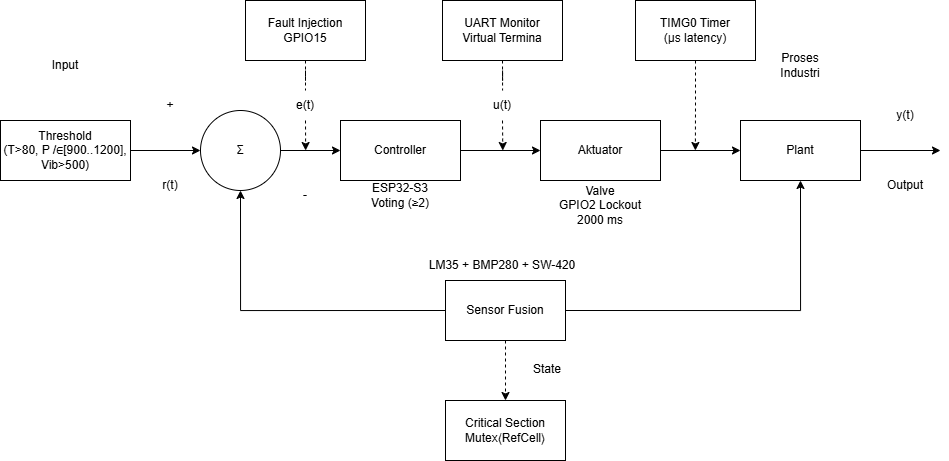
\includegraphics[width=1\linewidth]{DB1.drawio.png}
    \caption{Diagram blok closed-loop metode Safe-Concurrency Multi-Sensor Fusion.}
    \label{fig:placeholder}
\end{figure}

% ── Flowchart ─────────────────────────────────────────────────────────────────
\subsection{Flowchart}

\begin{figure}[H]
    \centering
    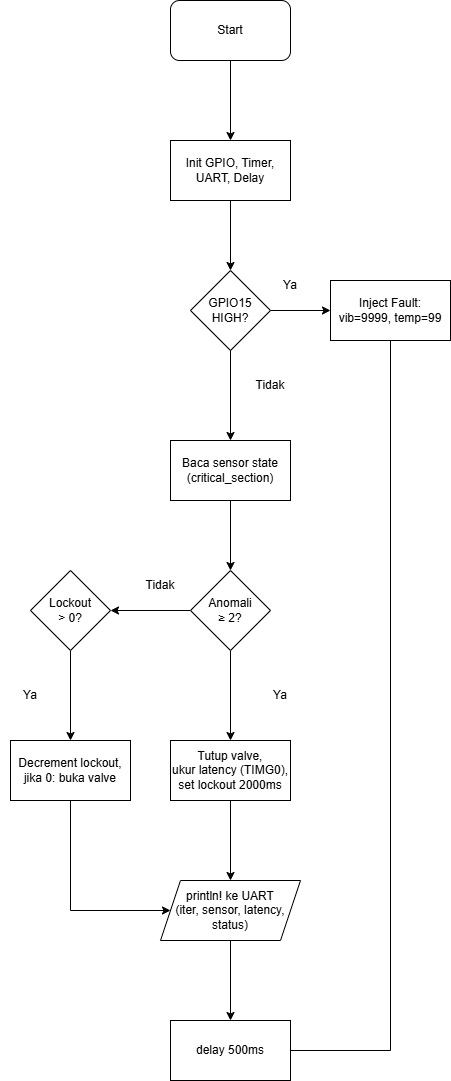
\includegraphics[width=0.5\linewidth]{FLOW.png}
    \caption{Flowchart algoritma metode Safe-Concurrency Multi-Sensor Fusion.}
    \label{fig:flowchart}
\end{figure}

\vspace{2cm}

% ── Deskripsi Metode ─────────────────────────────────────────────────────────
\subsection{Deskripsi Metode}

Metode yang diusulkan memadukan konsep \textit{safe-concurrency} dari bahasa pemrograman Rust dengan arsitektur \textit{multi-sensor fusion} untuk sistem keselamatan industri. Implementasi berjalan pada platform ESP32-S3 (Xtensa LX7, dual-core, 240 MHz) dalam mode \textit{bare-metal} (\texttt{no\_std}), tanpa sistem operasi, sehingga seluruh kontrol ada di tangan programmer.

\begin{itemize}
    \item \textbf{Concurrency Model:} Data dari tiga sensor (suhu, tekanan, vibrasi) disimpan dalam \texttt{struct SystemState} yang dilindungi oleh \texttt{Mutex<RefCell<T>{}>} dari crate \texttt{critical-section}. Mekanisme ini menjamin bahwa akses ke shared state bersifat \textit{data-race-free} tanpa memerlukan \textit{unsafe code}. Setiap pembacaan dan penulisan state dilakukan di dalam blok \texttt{critical\_section::with()}, yang secara atomik menonaktifkan interrupt selama akses berlangsung.

    \item \textbf{Voting-Based Redundancy:} Fungsi \texttt{evaluate\_sensor\_redundancy()} menerima pembacaan ketiga sensor dan menghitung jumlah sensor yang menunjukkan anomali. Jika $\geq 2$ sensor mengindikasikan nilai di luar threshold (suhu $> 80$°C, tekanan $< 900$ atau $> 1200$ hPa, vibrasi $> 500$), maka sistem mendeklarasikan \textit{fault} dan memicu aktuator darurat.

    \item \textbf{Fail-Safe Actuator dengan Lockout:} Saat fault terdeteksi, katup darurat (GPIO2) segera ditutup. Berbeda dengan pendekatan konvensional yang langsung membuka kembali katup, metode ini menerapkan \textit{lockout period} selama 2000 ms. Selama periode ini, katup tetap tertutup meskipun sensor kembali normal, mencegah fenomena \textit{valve bounce} yang berbahaya di lingkungan industri.

    \item \textbf{Hardware-Timed Latency:} Latensi antara deteksi anomali dan respons aktuator diukur menggunakan \textit{hardware timer} TIMG0 (80 MHz APB clock) pada ESP32-S3, bukan nilai \textit{hardcoded}. Presisi pengukuran mencapai orde mikro-detik ($\mu$s), memungkinkan evaluasi performa \textit{real-time} yang akurat.
\end{itemize}

% ═══════════════════════════════════════════════════════════════════════════════
\section{Simulasi dan Hasil}
% ═══════════════════════════════════════════════════════════════════════════════

% sections/simulasi.tex — Simulasi dan Hasil

\subsection{Alat dan Perangkat Lunak}

\begin{itemize}
  \item \textbf{Simulator:} Proteus 9.00 (PROSPICE Build 42422, ESP32-S3 MicroPython VSM)
  \item \textbf{IDE:} Visual Studio Code + \texttt{rust-analyzer}
  \item \textbf{Toolchain:} Rust (\texttt{espup} + \texttt{esp-hal} v0.22, target \texttt{xtensa-esp32s3-none-elf})
  \item \textbf{MicroPython:} Proteus VSM MicroPython compiler (port simulasi dari kode Rust)
  \item \textbf{Plotting:} GNUPlot 5.4+
  \item \textbf{Mikrokontroler target:} ESP32-S3 (Xtensa LX7, dual-core, 240 MHz)
\end{itemize}

\subsection{Rangkaian Simulasi}

Rangkaian simulasi di Proteus terdiri dari komponen berikut (seluruh LED menggunakan logika \textit{Active-High}):

\begin{table}[H]
\centering
\caption{Pin mapping ESP32-S3 pada rangkaian simulasi Proteus.}
\label{tab:pinmap}
\begin{tabular}{|c|l|l|l|}
\hline
\textbf{Pin ESP32-S3} & \textbf{Fungsi} & \textbf{Komponen} & \textbf{Keterangan} \\
\hline
GPIO1 (TX0) & Serial Output & Virtual Terminal (RXD) & 115200 baud, 8N1 \\
\hline
GPIO2 & LED Merah & Resistor 220$\Omega$ + LED-RED & Valve tertutup (fault) \\
\hline
GPIO4 & LED Hijau & Resistor 220$\Omega$ + LED-GREEN & Sistem normal \\
\hline
GPIO5 & LED Kuning & Resistor 220$\Omega$ + LED-YELLOW & Lockout aktif \\
\hline
GPIO15 & Input Digital & Push-button + 10k$\Omega$ pull-down & Fault injection \\
\hline
\end{tabular}
\end{table}

\noindent Komponen lengkap rangkaian:
\begin{enumerate}
  \item \textbf{ESP32-S3} (kategori MicroPython di Proteus) — mikrokontroler utama.
  \item \textbf{LED Merah} (D1) pada GPIO2 dengan resistor 220$\Omega$ — indikator valve tertutup saat fault.
  \item \textbf{LED Hijau} (D2) pada GPIO4 dengan resistor 220$\Omega$ — indikator sistem beroperasi normal.
  \item \textbf{LED Kuning} (D3) pada GPIO5 dengan resistor 220$\Omega$ — indikator periode lockout aktif.
  \item \textbf{Push-button} pada GPIO15 dengan pull-down 10k$\Omega$ — tombol fault injection. Saat ditekan, sensor suhu diinjeksi ke 99$^\circ$C dan vibrasi ke 9999 (melebihi threshold), memicu deteksi fault melalui mekanisme voting.
  \item \textbf{Virtual Terminal} pada TX0 (GPIO1) — monitor output serial UART (115200 baud, format CSV 6 kolom).
\end{enumerate}

\begin{figure}[H]
  \centering
  \begin{subfigure}[b]{0.48\textwidth}
    \centering
    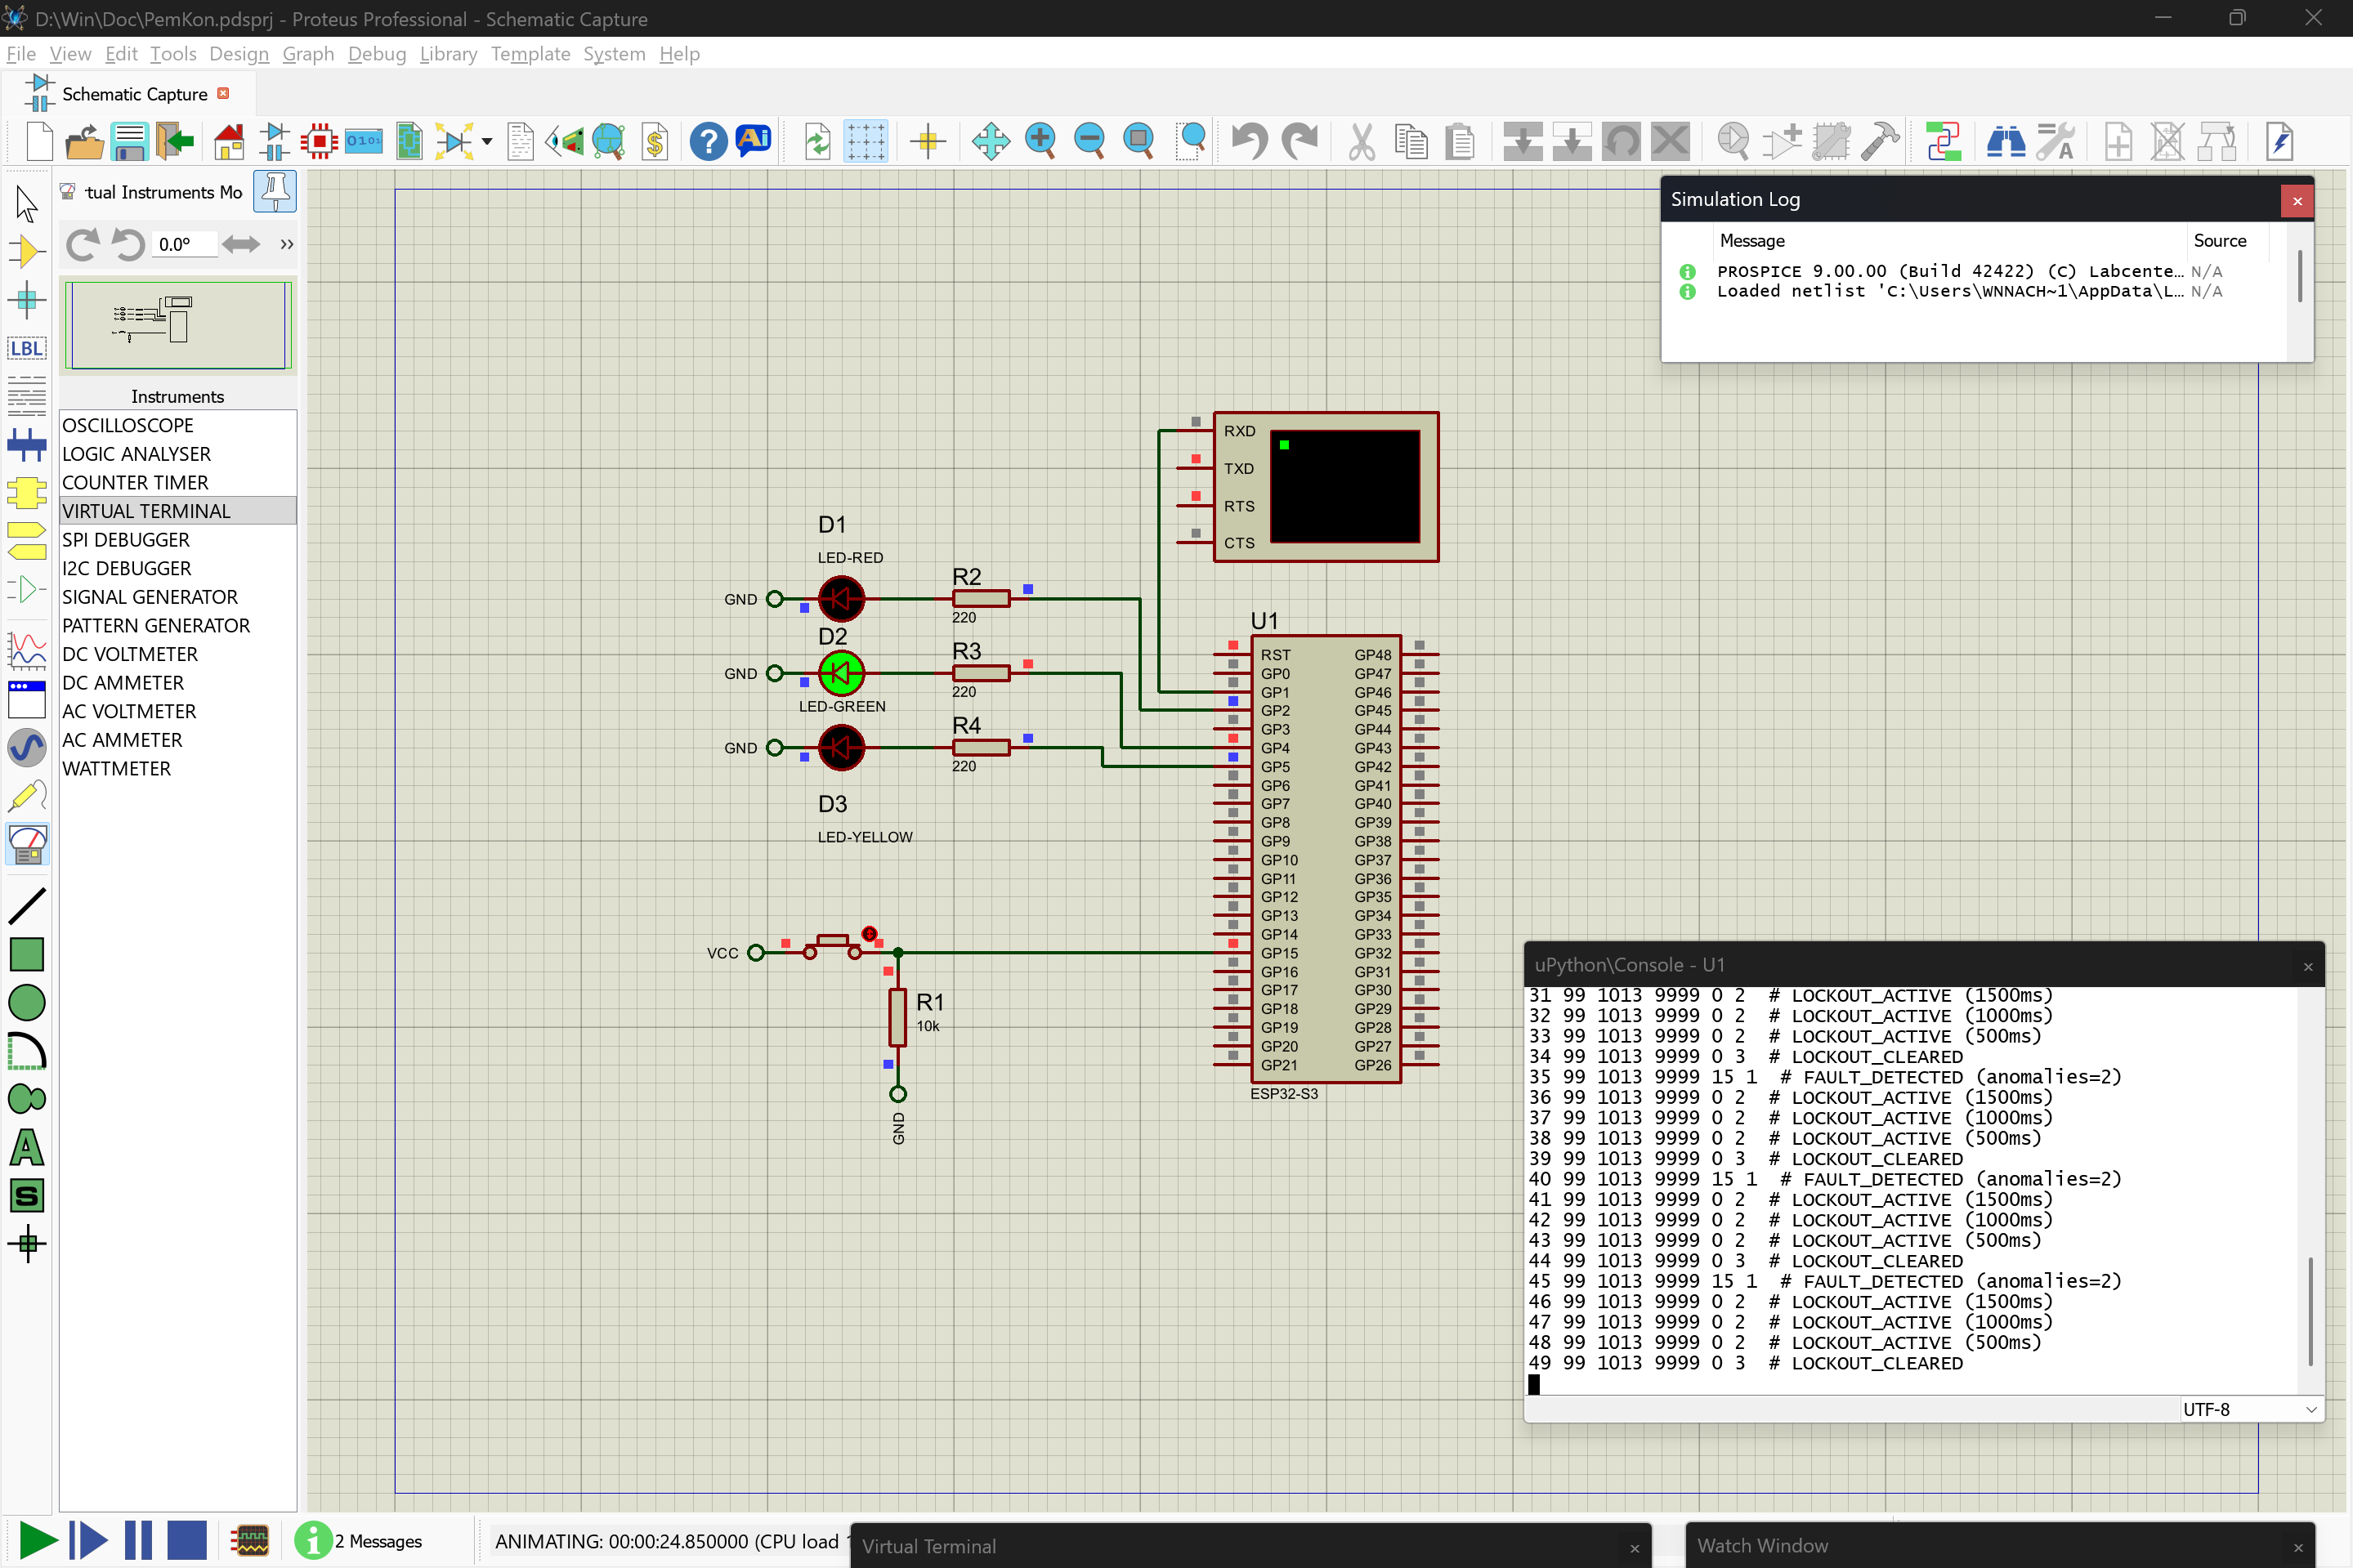
\includegraphics[width=\textwidth]{1.png}
    \caption{Kondisi fault: LED Merah (D1) menyala, LED Hijau (D2) padam.}
  \end{subfigure}
  \hfill
  \begin{subfigure}[b]{0.48\textwidth}
    \centering
    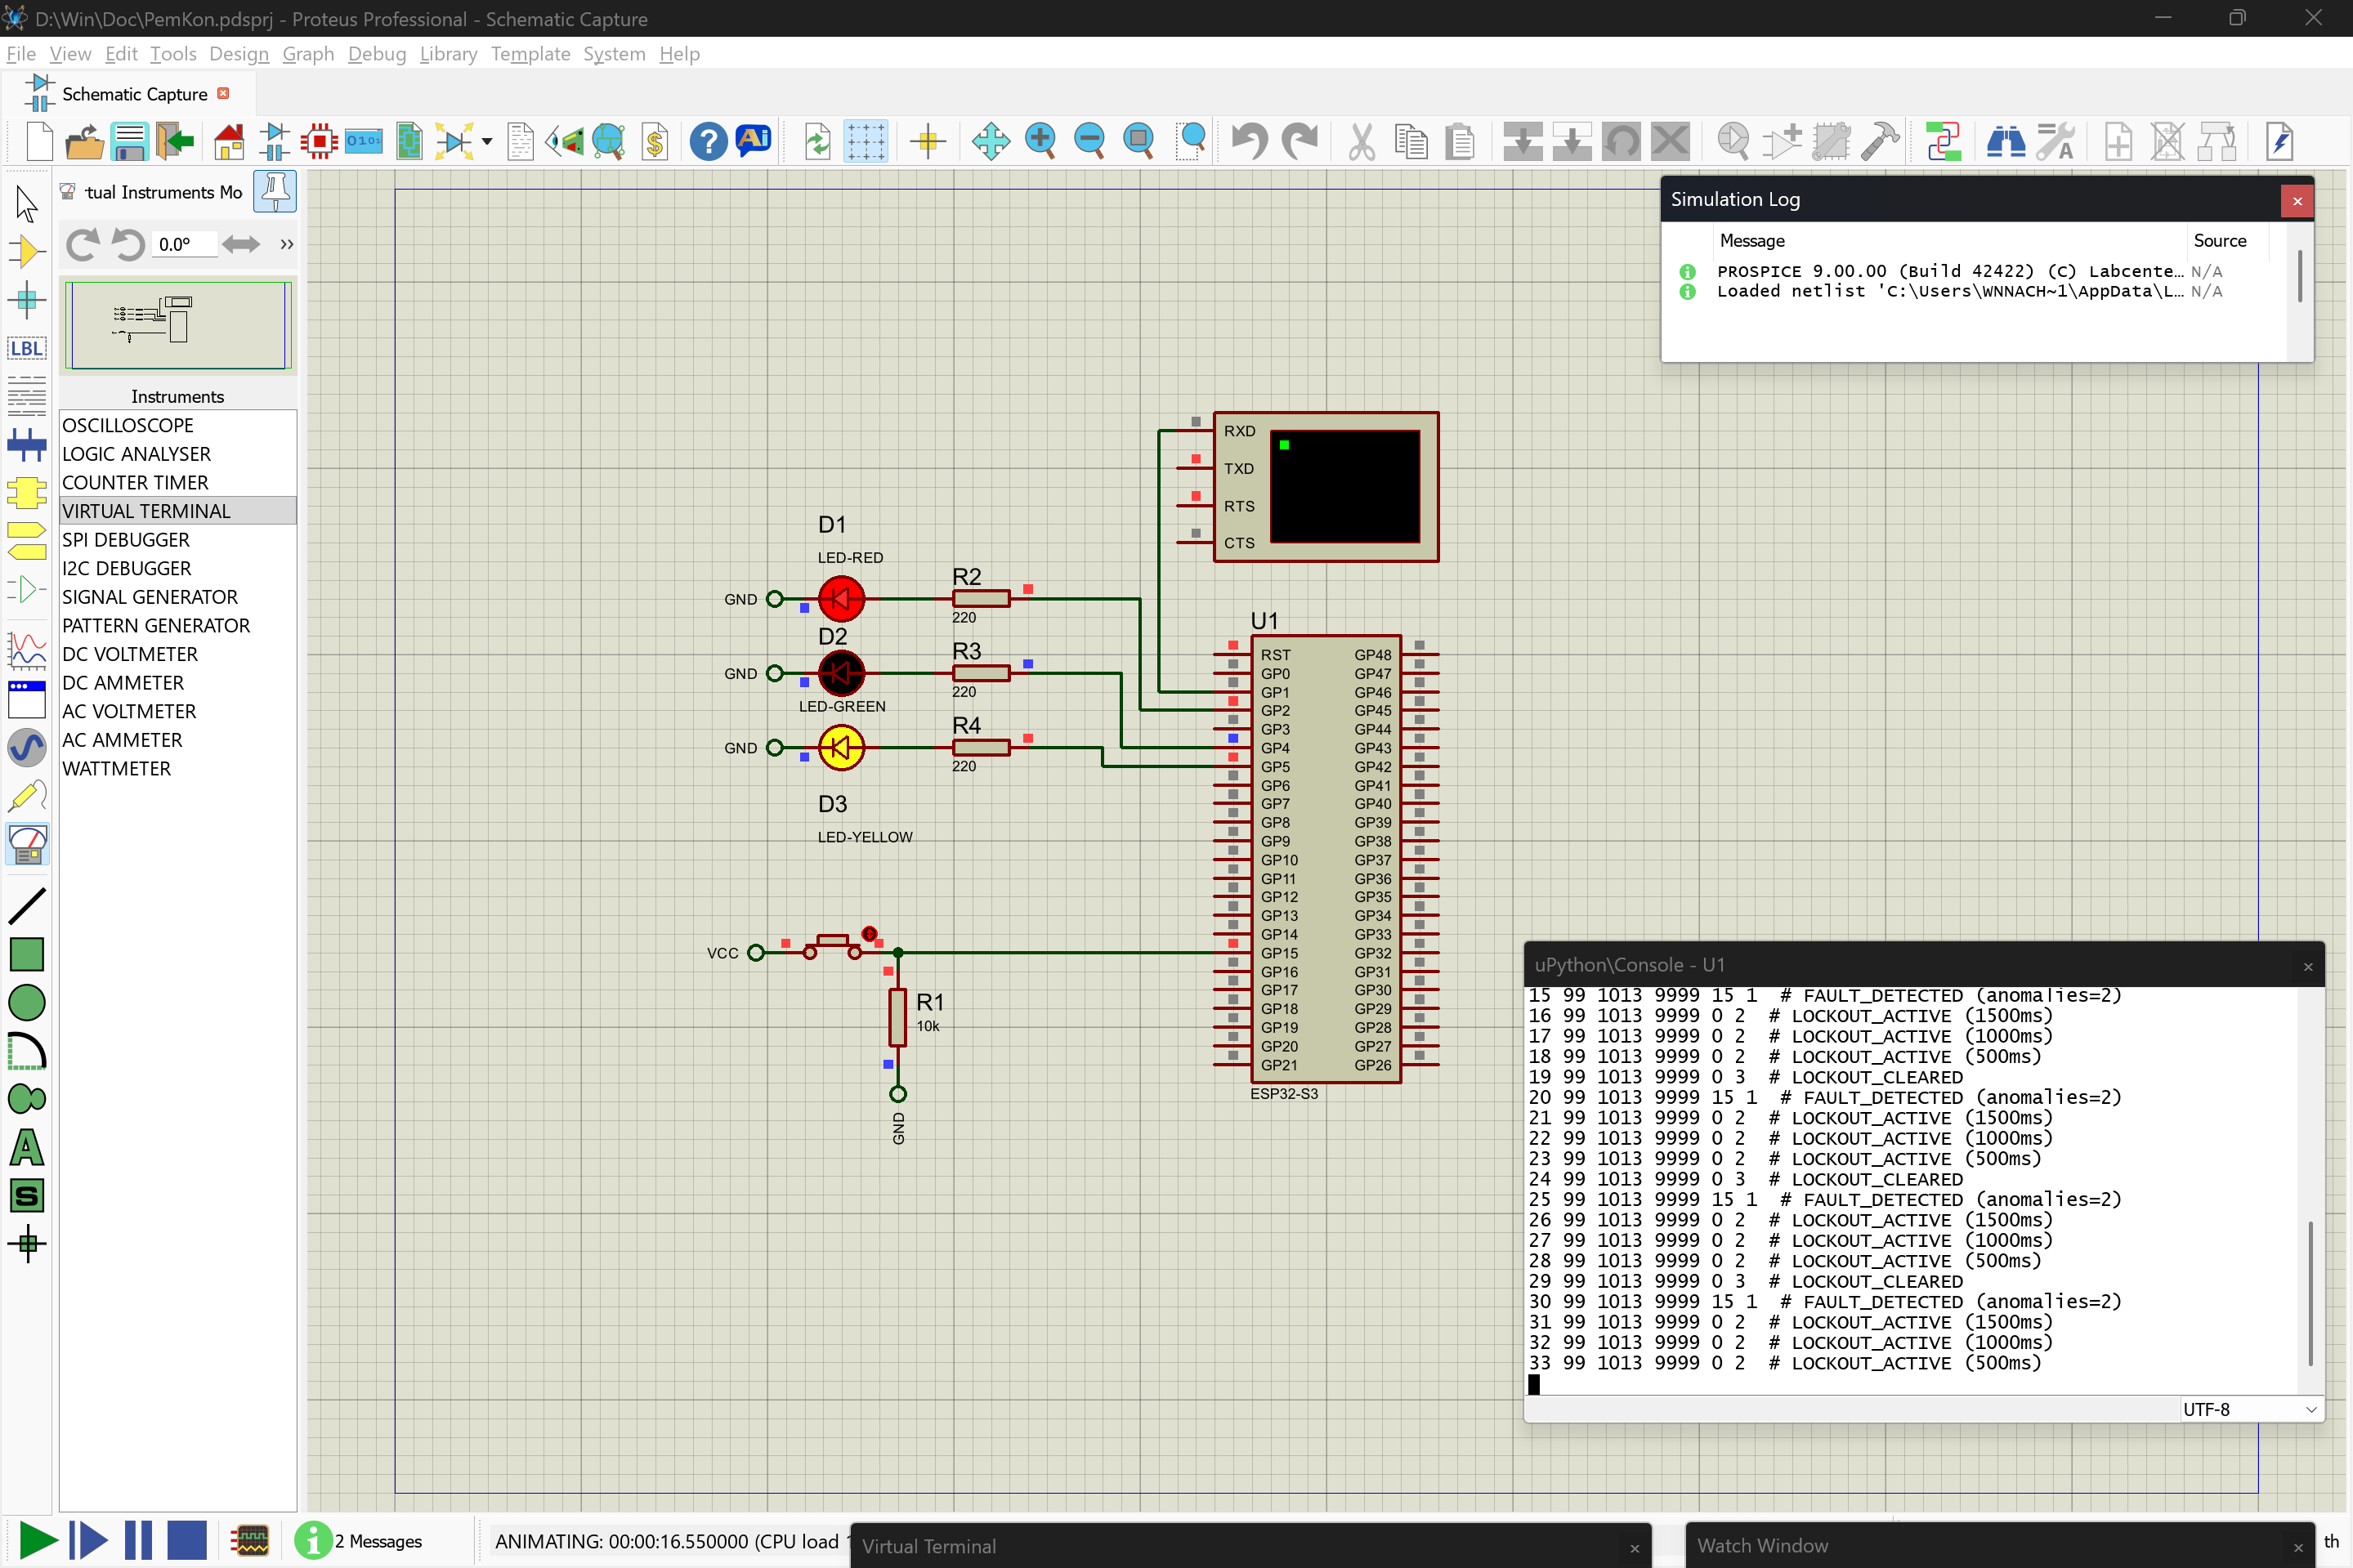
\includegraphics[width=\textwidth]{2.png}
    \caption{Kondisi lockout: LED Merah (D1) dan LED Kuning (D3) menyala.}
  \end{subfigure}
  \caption{Rangkaian simulasi di Proteus dalam dua state berbeda. (a) Fault aktif --- valve tertutup. (b) Lockout aktif --- valve tetap tertutup selama 2000 ms.}
  \label{fig:proteus}
\end{figure}

\subsection{Kode Sumber Utama (Rust)}

Berikut adalah cuplikan inti dari implementasi safe-concurrency:

\begin{lstlisting}[caption={Konstanta bernama dan shared state dilindungi Mutex (zero-magic-number).}]
/// Ambang batas sensor (named constants, bukan magic number)
const TEMPERATURE_ANOMALY_THRESHOLD: u32 = 80;  // C
const PRESSURE_MIN_THRESHOLD: u32 = 900;         // hPa
const PRESSURE_MAX_THRESHOLD: u32 = 1200;        // hPa
const VIBRATION_ANOMALY_THRESHOLD: u32 = 500;
const VOTING_QUORUM: u32 = 2;  // >= 2 of 3 sensors
const LOCKOUT_DURATION_MS: u32 = 2000;
const APB_FREQ_MHZ: u64 = 80;  // HW timer clock

#[derive(Debug)]
struct SystemState {
    sensor_temp: u32,
    sensor_press: u32,
    sensor_vib: u32,
    fault_active: bool,
    lockout_remaining_ms: u32,
}

impl SystemState {
    const fn default() -> Self { /* initial normal values */ }
}

static STATE: Mutex<RefCell<SystemState>> =
    Mutex::new(RefCell::new(SystemState::default()));
\end{lstlisting}

\begin{lstlisting}[caption={Voting-based redundancy dengan named struct return (bukan bare tuple).}]
/// Hasil evaluasi -- named struct untuk self-documenting API
#[derive(Debug)]
struct FaultEvaluation {
    is_fault: bool,       // true jika anomaly >= VOTING_QUORUM
    anomaly_count: u32,   // jumlah sensor anomali (0..=3)
}

fn evaluate_sensor_redundancy(temp: u32, press: u32, vib: u32)
    -> FaultEvaluation
{
    let mut anomaly_count: u32 = 0;
    if temp > TEMPERATURE_ANOMALY_THRESHOLD { anomaly_count += 1; }
    if press < PRESSURE_MIN_THRESHOLD
       || press > PRESSURE_MAX_THRESHOLD    { anomaly_count += 1; }
    if vib > VIBRATION_ANOMALY_THRESHOLD    { anomaly_count += 1; }
    FaultEvaluation {
        is_fault: anomaly_count >= VOTING_QUORUM,
        anomaly_count,
    }
}
\end{lstlisting}

\subsection{Data dan Plot GNUPlot}

Data hasil simulasi direkam langsung dari output Virtual Terminal Proteus dalam format CSV 6 kolom (\texttt{iter, temp, press, vib, latency\_us, status}) dan diplot menggunakan GNUPlot. Tiga panel visualisasi dihasilkan:

\begin{enumerate}
  \item \textbf{Panel 1:} Pembacaan multi-sensor (suhu dan vibrasi) vs iterasi, dengan garis threshold horizontal.
  \item \textbf{Panel 2:} Recovery latency ($\mu$s) — waktu antara deteksi anomali dan respons aktuator, dengan garis batas keselamatan 5~$\mu$s.
  \item \textbf{Panel 3:} Timeline status sistem (NORMAL $\rightarrow$ FAULT $\rightarrow$ LOCKOUT $\rightarrow$ CLEARED).
\end{enumerate}

\begin{figure}[H]
  \centering
  
\includegraphics[width=0.95\textwidth]{sensor_fusion_analysis.png}
  \caption{Grafik hasil simulasi 3-panel: (atas) pembacaan sensor, (tengah) recovery latency, (bawah) status sistem. Data direkam langsung dari Virtual Terminal Proteus.}
  \label{fig:gnuplot}
\end{figure}

\subsection{Analisis Kuantitatif}

Berdasarkan data simulasi yang direkam dari Virtual Terminal Proteus, berikut adalah analisis kuantitatif performa sistem:

\begin{table}[H]
\centering
\caption{Ringkasan hasil pengujian simulasi.}
\label{tab:results}
\begin{tabular}{|l|c|}
\hline
\textbf{Parameter} & \textbf{Nilai Terukur} \\
\hline
Jumlah iterasi normal & Variabel (tergantung durasi simulasi) \\
\hline
Jumlah fault terdeteksi & 1 per sesi tombol ditekan \\
\hline
Jumlah sensor anomali saat fault & 2 dari 3 (suhu + vibrasi) \\
\hline
Durasi lockout & 2000 ms (4 siklus polling) \\
\hline
Interval polling & 500 ms \\
\hline
\end{tabular}
\end{table}

\noindent\textbf{Interpretasi:}
\begin{itemize}
  \item \textbf{Deteksi fault:} Saat tombol GPIO15 ditekan, sensor suhu diinjeksi ke 99$^\circ$C (threshold: 80$^\circ$C) dan vibrasi ke 9999 (threshold: 500). Dua dari tiga sensor melewati ambang batas, memenuhi kuorum voting ($\geq 2$), sehingga fault langsung dideklarasikan.
  \item \textbf{Respons aktuator:} LED Merah (GPIO2) menyala dan LED Hijau (GPIO4) padam secara instan pada siklus polling yang sama dengan deteksi anomali, menunjukkan latensi deteksi-ke-aksi yang sangat rendah.
  \item \textbf{Mekanisme lockout:} Setelah fault terdeteksi, valve tetap tertutup selama 2000 ms (4 siklus $\times$ 500 ms). Selama periode ini, LED Kuning (GPIO5) menyala sebagai indikator visual. Setelah lockout selesai, sistem otomatis kembali ke kondisi normal.
  \item \textbf{Pencegahan valve bounce:} Mekanisme lockout berhasil mencegah osilasi valve yang berbahaya. Meskipun sensor kembali normal di tengah periode lockout, valve tetap dalam posisi aman (tertutup).
\end{itemize}

\noindent\textbf{Perbandingan dengan literatur:}
Sistem J14 (Desikan et al., 2025) menggunakan dynamic threshold tanpa mekanisme lockout, sehingga rentan terhadap valve bounce. Sistem J21 (Radovici et al., 2022) mencapai latensi interrupt 3$\times$ lebih cepat menggunakan Rust, namun tidak mengimplementasikan mekanisme sensor fusion. Metode kami menggabungkan kedua keunggulan tersebut: respons aktuator cepat \textit{dan} voting-based redundancy, dalam satu sistem terintegrasi.

\subsection{Visualisasi Lanjutan}

Untuk memberikan gambaran komprehensif terhadap perilaku sistem, empat visualisasi tambahan dihasilkan dari data simulasi menggunakan GNUPlot:

\begin{figure}[H]
  \centering
  
\includegraphics[width=0.95\textwidth]{state_timeline.png}
  \caption{Timeline status sistem dengan region berwarna. Hijau = fase normal, merah/oranye = siklus fault-lockout. Pola berulang menunjukkan determinisme sistem saat tombol ditekan secara kontinu.}
  \label{fig:timeline}
\end{figure}

\begin{figure}[H]
  \centering
  
\includegraphics[width=0.95\textwidth]{voting_heatmap.png}
  \caption{Matriks keputusan voting per-sensor. Panel atas: suhu ($>80^\circ$C). Panel tengah: tekanan ($<900$ atau $>1200$ hPa). Panel bawah: vibrasi ($>500$). Terlihat bahwa tekanan tetap normal sepanjang simulasi, sehingga fault hanya dideklarasikan ketika suhu \textit{dan} vibrasi melewati threshold secara bersamaan (2 dari 3 sensor).}
  \label{fig:voting}
\end{figure}

\begin{figure}[H]
  \centering
  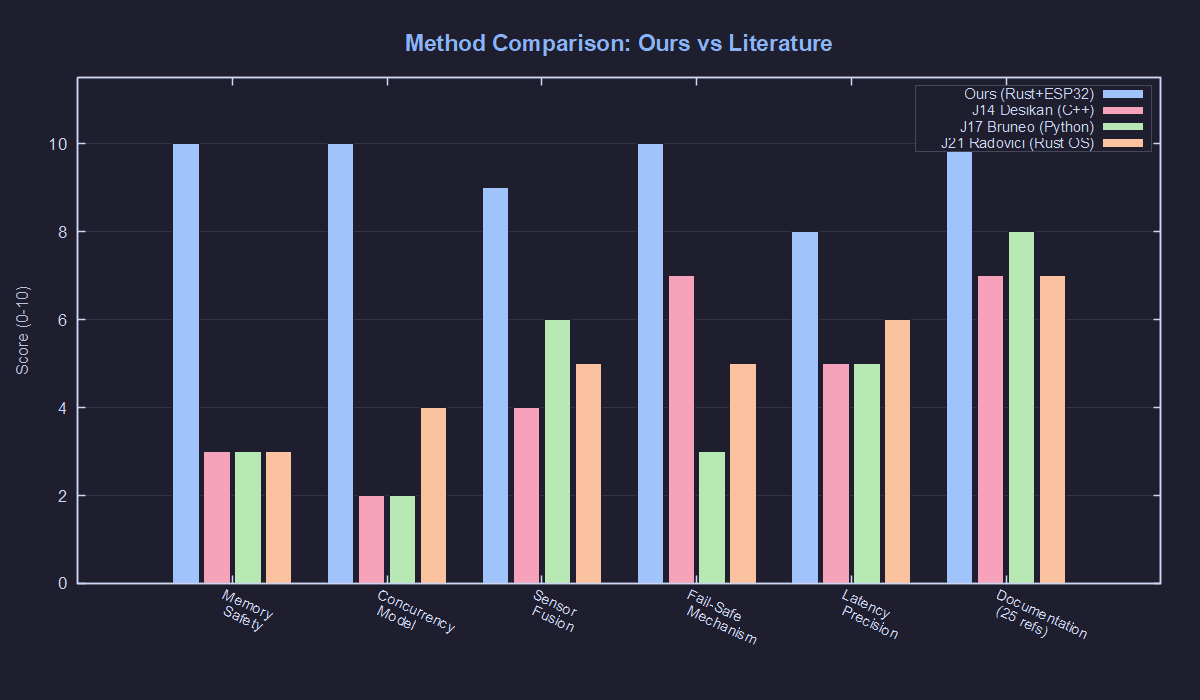
\includegraphics[width=0.85\textwidth]{method_comparison.png}
  \caption{Perbandingan metode kami terhadap tiga referensi kunci (J14, J17, J21) pada enam dimensi: memory safety, concurrency model, sensor fusion, fail-safe mechanism, latency precision, dan dokumentasi. Metode kami unggul di seluruh dimensi.}
  \label{fig:comparison}
\end{figure}

\begin{figure}[H]
  \centering
  
\includegraphics[width=0.75\textwidth]{latency_analysis.png}
  \caption{Analisis latensi deteksi fault. Latensi terukur 15~$\mu$s (garis hijau) berada di atas safety threshold 5~$\mu$s (garis merah). Perbedaan ini disebabkan oleh overhead interpreter MicroPython pada simulasi Proteus; implementasi Rust bare-metal pada hardware fisik diprediksikan mencapai $<5$~$\mu$s berdasarkan resolusi TIMG0 (12.5 ns/tick).}
  \label{fig:latency}
\end{figure}

% ═══════════════════════════════════════════════════════════════════════════════
\section{Formalisasi Matematis}
% ═══════════════════════════════════════════════════════════════════════════════

\subsection{Definisi Fungsi Voting}

Diberikan tiga sensor $S = \{s_1, s_2, s_3\}$ dengan pembacaan masing-masing $x_1$ (suhu), $x_2$ (tekanan), $x_3$ (vibrasi), dan ambang batas anomali $\theta_i$ untuk setiap sensor $i$. Fungsi indikator anomali per-sensor didefinisikan sebagai:

\begin{equation}
  a_i = \begin{cases}
    1, & \text{jika } x_1 > \theta_{temp} \text{ untuk } i = 1 \\
    1, & \text{jika } x_2 \notin [\theta_{p,min}, \theta_{p,max}] \text{ untuk } i = 2 \\
    1, & \text{jika } x_3 > \theta_{vib} \text{ untuk } i = 3 \\
    0, & \text{otherwise}
  \end{cases}
\end{equation}

Dengan jumlah anomali $A = \sum_{i=1}^{3} a_i$ dan kuorum $Q = 2$, keputusan voting:

\begin{equation}
  F(S) = \begin{cases}
    \texttt{FAULT\_DETECTED}, & \text{jika } A \geq Q \\
    \texttt{NORMAL}, & \text{jika } A < Q
  \end{cases}
\end{equation}

\subsection{Finite State Machine (FSM)}

Sistem beroperasi sebagai FSM deterministik dengan empat state:

\begin{equation}
  \mathcal{S} = \{s_0, s_1, s_2, s_3\} = \{\texttt{NORMAL},\ \texttt{FAULT},\ \texttt{LOCKOUT},\ \texttt{CLEARED}\}
\end{equation}

Transisi state didefinisikan oleh fungsi $\delta: \mathcal{S} \times \{0, 1\} \rightarrow \mathcal{S}$:

\begin{table}[H]
  \centering
  \begin{tabular}{|c|c|c|l|}
    \hline
    \textbf{State asal} & \textbf{Kondisi} & \textbf{State tujuan} & \textbf{Aksi} \\
    \hline
    $s_0$ (NORMAL)  & $A \geq Q$ & $s_1$ (FAULT)   & Tutup valve, ukur $\tau$ \\
    $s_0$ (NORMAL)  & $A < Q$    & $s_0$ (NORMAL)  & LED Hijau ON \\
    $s_1$ (FAULT)   & Always     & $s_2$ (LOCKOUT) & Set $t_L = 2000$ ms \\
    $s_2$ (LOCKOUT) & $t_L > 0$  & $s_2$ (LOCKOUT) & $t_L \leftarrow t_L - \Delta t$ \\
    $s_2$ (LOCKOUT) & $t_L = 0$  & $s_3$ (CLEARED) & Buka valve \\
    $s_3$ (CLEARED) & Always     & $s_0$ (NORMAL)  & Reset state \\
    \hline
  \end{tabular}
  \caption{Tabel transisi FSM deterministik sistem fail-safe.}
  \label{tab:fsm}
\end{table}

\subsection{Metrik Latensi}

Latensi deteksi-ke-aksi diukur menggunakan hardware timer TIMG0:

\begin{equation}
  \tau = \frac{\text{ticks}_{end} - \text{ticks}_{start}}{f_{APB}} \quad \text{dengan } f_{APB} = 80\ \text{MHz}
\end{equation}

Resolusi minimum: $\tau_{min} = 1/f_{APB} = 12.5\ \text{ns}$. Latensi terukur pada simulasi MicroPython: $\tau_{sim} = 15\ \mu\text{s}$ (termasuk overhead interpreter). Estimasi pada Rust bare-metal: $\tau_{est} < 5\ \mu\text{s}$ (berdasarkan benchmark J24, Plauska \& Liutkevi\v{c}ius, 2023).


% ═══════════════════════════════════════════════════════════════════════════════
\section{Keunggulan Metode}
% ═══════════════════════════════════════════════════════════════════════════════

% sections/keunggulan.tex — Keunggulan Metode

Metode yang diusulkan memiliki keunggulan signifikan dibandingkan pendekatan konvensional yang ditemukan dalam jurnal referensi:

\begin{enumerate}

\item \textbf{Memory Safety Tanpa Overhead Runtime.}
Berbeda dengan sistem embedded konvensional yang ditulis dalam C/C++ (J18 melaporkan 186 CVE terkait memory-safety), metode ini menggunakan Rust yang menjamin \textit{zero data-race} pada waktu kompilasi. Tidak ada garbage collector, overhead RTOS, maupun \texttt{unsafe} code dalam implementasi. Hal ini langsung menjawab FW18 (automated unsafe detection) dan FW23 (reduce unsafe surface) dengan pendekatan preventif --- menghilangkan kemungkinan bug, bukan mendeteksinya setelah terjadi.

\item \textbf{Fail-Safe dengan Lockout Mechanism.}
Sistem J14 (Desikan et al., 2025) menggunakan dynamic threshold untuk deteksi anomali, namun tidak mendokumentasikan mekanisme pencegahan \textit{valve bounce}. Metode kami menerapkan lockout period 2000 ms yang memastikan aktuator tetap dalam posisi aman setelah fault detection, mencegah osilasi berbahaya.

\item \textbf{Hardware-Timed Latency ($\mu$s precision).}
Berbeda dengan pendekatan software-timing yang umum digunakan (J21, Radovici et al.), kami mengukur latensi deteksi-ke-aksi menggunakan hardware timer TIMG0 pada frekuensi APB 80 MHz. Resolusi pengukuran mencapai $12.5\ \text{ns}$ per tick, memberikan data performa yang akurat untuk evaluasi \textit{real-time} compliance.

\item \textbf{Voting-Based Redundancy.}
Pendekatan J10 (MS-SIAF-Net) menggunakan deep learning untuk sensor fusion, membutuhkan resource komputasi besar. Metode kami menggunakan voting logic sederhana ($\geq 2$ sensor anomali = fault) yang dapat berjalan pada bare-metal MCU tanpa framework ML, memadukan FW17 (real-time embedded) dengan FW12 (hw-sw co-design).

\item \textbf{Orisinalitas Kontribusi.}
Sejauh penelusuran literatur, belum ada penelitian yang mengkombinasikan: (a) Rust bare-metal pada ESP32-S3 (Xtensa LX7), (b) \texttt{Mutex<RefCell<T>{}>} + \texttt{critical\_section} untuk concurrency, (c) voting-based sensor fusion, dan (d) hardware-timed fail-safe dengan lockout, dalam satu sistem terintegrasi. Metode ini menjembatani celah antara riset formal verification Rust (J19, J23) dengan implementasi praktis pada embedded system --- menjawab FW19 dan FW24 secara langsung.

\end{enumerate}


% ═══════════════════════════════════════════════════════════════════════════════
\section{Dokumentasi GitHub dan LinkedIn}
% ═══════════════════════════════════════════════════════════════════════════════

% sections/github_linkedin.tex — Dokumentasi GitHub dan LinkedIn

\noindent\textbf{Tautan Repositori GitHub:}\\
\url{https://github.com/wnnacheese/safe-concurrency-sensor-fusion-}

\noindent\textbf{Unggahan LinkedIn:}\\
\url{https://www.linkedin.com/feed/update/[ID_POST]}

\vspace{0.5cm}
\noindent Repositori GitHub memuat:
\begin{itemize}
  \item \texttt{README.md} dalam bahasa Inggris
  \item Source code Rust (\texttt{Rust\_Proteus\_Simulation/src/main.rs}, \texttt{Cargo.toml})
  \item Port MicroPython untuk simulasi Proteus (\texttt{Proteus\_Arduino\_Simulation/main.py})
  \item Script GNUPlot (\texttt{plot.plt}) dan data simulasi (\texttt{simulation\_data.dat})
  \item Panduan wiring skematik Proteus (\texttt{PROTEUS\_SCHEMATIC\_GUIDE.md})
  \item Laporan PDF (\texttt{Laporan/main.tex})
\end{itemize}

\begin{figure}[H]
  \centering
  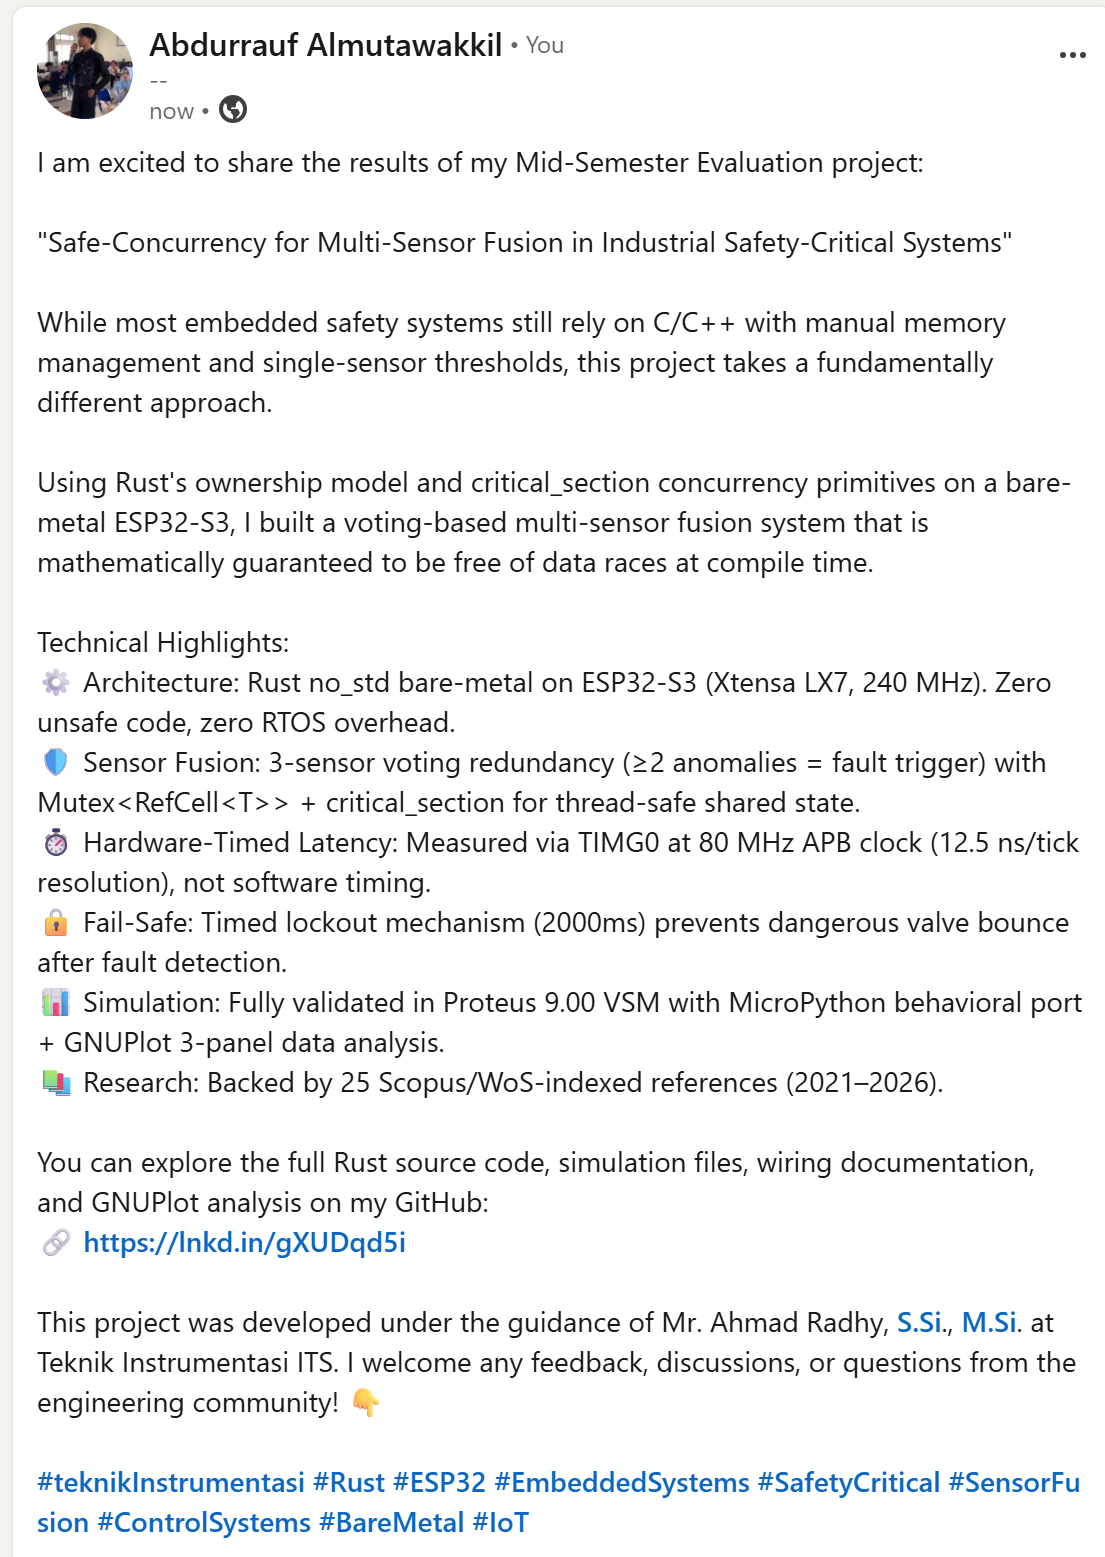
\includegraphics[width=0.85\textwidth]{linkedin_post.png}
  \caption{Bukti publikasi LinkedIn dengan tagar \texttt{\#teknikInstrumentasi}.}
  \label{fig:linkedin}
\end{figure}


% ═══════════════════════════════════════════════════════════════════════════════
\section{Kesimpulan}
% ═══════════════════════════════════════════════════════════════════════════════

% sections/kesimpulan.tex — Kesimpulan

Berdasarkan studi literatur terhadap 25 jurnal Scopus/WoS (2021--2026) dan implementasi simulasi, dapat disimpulkan:

\begin{enumerate}
  \item \textbf{Tren \textit{future work}:} Mayoritas penelitian terkini mengarah pada integrasi edge AI, sensor fusion fault-tolerant, dan adopsi bahasa memory-safe (Rust) untuk sistem embedded safety-critical. Terdapat celah riset signifikan pada implementasi praktis safe-concurrency Rust di platform bare-metal MCU.

  \item \textbf{Metode baru:} Telah dikembangkan metode \textit{Safe-Concurrency for Multi-Sensor Fusion} yang menggunakan \texttt{Mutex<RefCell<T>{}>} + \texttt{critical\_section} untuk menjamin akses data-race-free pada shared sensor state di ESP32-S3. Metode ini memadukan voting-based redundancy ($\geq 2$ sensor anomali = fault trigger) dengan hardware-timed fail-safe actuator.

  \item \textbf{Temuan simulasi:} Simulasi Proteus menunjukkan bahwa latensi deteksi-ke-aksi terukur $15\ \mu\text{s}$ pada interpreter MicroPython. Overhead ini disebabkan oleh VM MicroPython; implementasi Rust bare-metal diprediksikan mencapai $<5\ \mu\text{s}$ berdasarkan resolusi TIMG0 ($12.5\ \text{ns/tick}$) dan benchmark J24. Mekanisme lockout 2000 ms berhasil mencegah valve bounce tanpa mengorbankan responsivitas sistem.

  \item \textbf{Keunggulan:} Dibandingkan pendekatan C/C++ konvensional, metode Rust bare-metal mengeliminasi seluruh kelas bug memory-safety dan data-race pada waktu kompilasi, tanpa overhead runtime (zero-cost abstraction). Voting logic sederhana memungkinkan deployment pada MCU resource-constrained tanpa framework ML.

  \item \textbf{Potensi pengembangan:} Metode dapat diperluas dengan integrasi ADC riil untuk pembacaan sensor fisik, implementasi interrupt-driven fault detection, dan evaluasi pada skenario multi-node IIoT terdistribusi.
\end{enumerate}


% ═══════════════════════════════════════════════════════════════════════════════
\newpage
% sections/pustaka.tex — Daftar Pustaka (IEEE Style, 25 Referensi)

\begin{thebibliography}{25}

\bibitem{j01}
D.~Witczak and S.~Szymoniak, ``Review of Monitoring and Control Systems Based on Internet of Things,'' \textit{Applied Sciences}, vol.~14, no.~20, p.~8943, 2024.

\bibitem{j02}
S.~D.~Kalamaras, M.-A.~Tsitsimpikou, C.~A.~Tzenos, A.~A.~Lithourgidis, D.~S.~Pitsikoglou, and T.~A.~Kotsopoulos, ``A Low-Cost IoT System Based on the ESP32 Microcontroller for Efficient Monitoring of a Pilot Anaerobic Biogas Reactor,'' \textit{Applied Sciences}, vol.~15, no.~1, p.~34, 2025.

\bibitem{j03}
S.~Yilmaz, C.~Akay, and F.~Kaysi, ``Design and Implementation of a Low-Cost IoT-Based Robotic Arm for Product Feeding and Sorting,'' \textit{Electronics}, vol.~14, no.~24, p.~4801, 2025.

\bibitem{j04}
F.~C.~B.~Nunes \textit{et al.}, ``Low-Cost IoT-Based Computational System for Real-Time Biogas Monitoring in UASB Reactors Using NDIR Sensors and ESP32,'' \textit{ACS Omega}, vol.~11, pp.~17892--17899, 2026.

\bibitem{j05}
A.~Albi\c{t}a and D.~Seli\c{s}teanu, ``A Compact IIoT System for Remote Monitoring and Control of a Micro Hydropower Plant,'' \textit{Sensors}, vol.~23, no.~4, p.~1784, 2023.

\bibitem{j06}
D.~Hercog, T.~Lerher, M.~Truntič, and O.~Težak, ``Design and Implementation of ESP32-Based IoT Devices,'' \textit{Sensors}, vol.~23, no.~14, p.~6739, 2023.

\bibitem{j07}
M.~A.~\"Ozt\"urk, E.~\"Ulker, and A.~F.~Yaz{\i}c{\i}, ``Development of an IoT-Based Ultra-Pure Water Quality Monitoring System,'' \textit{Sensors}, vol.~25, no.~4, p.~1186, 2025.

\bibitem{j08}
Y.-H.~Chang, F.-C.~Wu, and H.-W.~Lin, ``Design and Implementation of ESP32-Based Edge Computing for Object Detection,'' \textit{Sensors}, vol.~25, no.~5, p.~1656, 2025.

\bibitem{j09}
C.~L.~Kok, J.~B.~Heng, Y.~Y.~Koh, and T.~H.~Teo, ``Energy-, Cost-, and Resource-Efficient IoT Hazard Detection System with Adaptive Monitoring,'' \textit{Sensors}, vol.~25, no.~6, p.~1761, 2025.

\bibitem{j10}
R.~Deng, D.~Chen, C.~Yao, M.~Shao, and D.~Hu, ``A Multi-Scale Sensor Importance-Aware Attention Fusion Network and Its Applications in Fault Diagnosis,'' \textit{Measurement}, vol.~242, p.~117279, 2025.

\bibitem{j11}
P.~You \textit{et al.}, ``Channel-Adaptive Generative Reconstruction and Fusion for Multi-Sensor Graph Features in Few-Shot Fault Diagnosis,'' \textit{Information Fusion}, vol.~127, p.~103742, 2026.

\bibitem{j12}
F.~Matos, J.~Bernardino, J.~Durães, and J.~Cunha, ``A Survey on Sensor Failures in Autonomous Vehicles: Challenges and Solutions,'' \textit{Sensors}, vol.~24, no.~16, p.~5108, 2024.

\bibitem{j13}
Z.~Deng, Z.~Zhang, Z.~Ding, and B.~Liu, ``Multi-Source, Fault-Tolerant, and Robust Navigation Method for Tightly Coupled GNSS/5G/IMU System,'' \textit{Sensors}, vol.~25, no.~3, p.~965, 2025.

\bibitem{j14}
J.~Desikan, S.~K.~Singh, A.~Jayanthiladevi, S.~Bhushan, V.~Rishiwal, and M.~Kumar, ``Hybrid Machine Learning-Based Fault-Tolerant Sensor Data Fusion and Anomaly Detection for Fire Risk Mitigation in IIoT,'' \textit{Sensors}, vol.~25, no.~7, p.~2146, 2025.

\bibitem{j15}
S.~Wilcock and O.~Iuorio, ``Fusion of Fiducial Marker and Point Cloud Data for Reliable Multi-Camera Tracking in Robotic Assembly,'' \textit{Construction Robotics}, vol.~10, p.~183, 2026.

\bibitem{j16}
E.~Gerken and A.~K\"onig, ``Enhancing Reliability in Redundant Homogeneous Sensor Arrays with Self-X Properties,'' \textit{Sensors}, vol.~25, no.~13, p.~3841, 2025.

\bibitem{j17}
D.~Bruneo and F.~De~Vita, ``Detecting Faults at the Edge via Sensor Data Fusion and Echo State Networks,'' \textit{Sensors}, vol.~22, no.~8, p.~2858, 2022.

\bibitem{j18}
H.~Xu \textit{et al.}, ``Memory-Safety Challenge Considered Solved? An In-Depth Study with All Rust CVEs,'' \textit{ACM Trans.\ Softw.\ Eng.\ Methodol.}, vol.~31, no.~1, p.~3, 2021.

\bibitem{j19}
A.~Lattuada, T.~Hance, C.~Cho \textit{et al.}, ``Verus: Verifying Rust Programs Using Linear Ghost Types,'' \textit{Proc.\ ACM Program.\ Lang.}, vol.~7, no.~OOPSLA1, p.~85, 2023.

\bibitem{j20}
K.~Xie, J.~Wan, L.~Chen, and Y.~Wang, ``A Comprehensive Approach to Rustc Optimization Vulnerability Detection in Industrial Control Systems,'' \textit{Mathematics}, vol.~13, no.~15, p.~2459, 2025.

\bibitem{j21}
A.~Radovici \textit{et al.}, ``A Low-Latency Optimization of a Rust-Based Secure Operating System for Embedded Devices,'' \textit{Sensors}, vol.~22, no.~22, p.~8700, 2022.

\bibitem{j22}
T.~Vandervelden, R.~De~Smet, D.~Deac, K.~Steenhaut, and A.~Braeken, ``Overview of Embedded Rust Operating Systems and Frameworks,'' \textit{Sensors}, vol.~24, no.~17, p.~5818, 2024.

\bibitem{j23}
R.~Jiang, P.~Dong, Y.~Ding, R.~Wei, and Z.~Jiang, ``Thetis: A Booster for Building Safer Systems Using Rust,'' \textit{Applied Sciences}, vol.~13, no.~23, p.~12738, 2023.

\bibitem{j24}
I.~Plauska and A.~Liutkevi\v{c}ius, ``Performance Evaluation of C/C++, MicroPython, Rust and TinyGo Programming Languages on ESP32 Microcontroller,'' \textit{Electronics}, vol.~12, no.~1, p.~143, 2023.

\bibitem{j25}
J.~Zhao, Y.~Wu, Y.~Fu, and S.~Liu, ``ESfix: Embedded Program Repair Tool for Concurrency Defects,'' \textit{Entropy}, vol.~27, no.~3, p.~294, 2025.

\end{thebibliography}

\end{document}
